\documentclass{deliverablereport}

\deliverable{hpc}{GAP-HPC-report}
\deliverydate{XX/YY/201Z}
\duedate{31/08/2019 (M48)}
\author{Author names}

\begin{document}
\maketitle
% This will be the abstract, fetched from the github description
\githubissuedescription

% write the report here

% Original list of sections and subsections created from
% https://github.com/OpenDreamKit/OpenDreamKit/issues/113

TODO: Write some preamble. Describe the structure of this report.

\section{Developments in the core GAP system}\label{core-gap}

This Section highlights some most important and relevant to
OpenDreamKit changes in the new GAP releases published during the
project. More detailed descriptions of each major and minor
GAP release, with links to the corresponding pull requests on GitHub,
are contained in the ``GAP - Changes from Earlier Versions''
manual, which is redistributed with GAP and also available on the GAP
website at \url{https://www.gap-system.org/Manuals/doc/changes/chap0.html}.
This work includes contributions from our external collaborators, whose
authorship could be seen from the version control history.

\subsection{GAP 4.8 (February 2016)}\label{gap-4.8}

GAP 4.8 was the first major release of GAP published
after the start of the OpenDreamKit project.
As a preparation for the future developments to support multithreading, 
some language extensions from the HPC-GAP project were backported to the 
GAP library to help to unify the codebase of both GAP 4 and HPC-GAP. 

This release also included some language extensions which would allow users to write
more efficient and readable code, such as support for \emph{partially variadic functions}
to allow function expressions like
\verb|function( a, b, c, x... ) ... end;|
which would require at least three arguments and assign the first 
three to \verb|a|, \verb|b| and \verb|c| and then a list containing 
any remaining ones to \verb|x|, and an ability to install (in the library 
or packages) methods for accessing lists using multiple indices 
and indexing into lists using indices other than positive small integers. 
Such methods could allow, for example, to support expressions like

{\small
\begin{verbatim}
m[1,2];
m[1,2,3] := x;
IsBound(m["a","b",Z(7)]);
Unbind(m[1][2,3])
\end{verbatim}
}

In addition, it also provided 
support for profiling, e.g. tracking how much time in spent on 
each line of GAP code. This can be used to show where code is spending 
a long time and also check which lines of code are even executed. Profiling
functions \verb|ProfileLineByLine| and \verb|CoverageLineByLine| in the core 
GAP system were accompanied by the {\sf Profiling} package by Christopher Jefferson 
(St Andrews) for transforming these profiles into a human-readable form.

GAP 4.8 had seven public releases between February 2016 and August 2017, and
was replaced by GAP 4.9.

\subsection{GAP 4.9 (May 2018)}\label{gap-4.9}

GAP 4.9 continued restructuring and modernising of the core GAP system.
For example, we removed our old home-grown big integer code, and instead always 
use the GMP based big integer code. This means that the GMP library 
now is a required dependency, not just an optional one. Note that GAP 
has been using GMP big integer arithmetic for a long time by default, 
and we also have been bundling GMP with GAP. So this change mostly 
removed code that was never in use for most users.

Next, GAP got a new build system, which resolved many issues with the old
system, and should be easier to maintain. Technical technical details
of the new build system are described in {\tt README.buildsys.md} from
the GAP source code. 

The next major change, which was enabled by the new build system, was 
merging the experimental code to support multithreaded programming in GAP, 
dubbed HPC-GAP, into the mainstream GAP system (for details, see
Subsection~\ref{hpc-gap}).

Along the line, many performance improvements have been made. For example,
GAP now supports constant variables, whose value cannot change anymore 
during runtime; the code using such constants can now be optimised by GAP.
The performance of GAP's sorting functions (such as Sort, SortParallel, 
etc.) has been substantially improved, in some examples by more than a 
factor of four: as a trivial example, compare the timing for 
{\tt Sort([1..100000000] * 0)}. %#609
The output and behaviour of the profiling system has been substantially improved
as well.

Many changes improving GAP usability by allowing to write more
efficient and readable code, e.g.

- In addition to supporting single argument lambda functions 
like \verb|a -> a+1|, GAP now supports lambdas with fewer or more 
than one argument, or even a variable number. 
E.g. \verb|{a,b} -> a+b| is a shorthand for \verb|function(a,b) return a+b; end|. % #490.

- Function calls, list accesses and records accesses now can be nested. 
For example, you can now write \verb|y := f().x;| 
(essentially equivalent to \verb|y := f();; y := y.x;|),
which previously would have resulted in an error, % #457 and #462

Debugging also became easier: in many cases GAP now outputs the filename 
and location of functions in helpful places, e.g. in error messages or when 
displaying compiled functions.

GAP 4.9 had three public releases between May and September 2019, and
was replaced by GAP 4.10.

\subsection{GAP 4.10 (November 2018)}\label{gap-4.10}

The release of GAP 4.9 with the new build system allowed to continue
further restructuring of the core GAP system and finalise a number of
earlier started changes in the GAP master branch, resulting in the 
next major release just several months later. GAP 4.10 is current version
of GAP, with the latest release being GAP 4.10.2, published in June 2019.

GAP 4.10 provides an experimental support for using the Julia garbage collector.
It is now possible to use the garbage collector of the Julia language 
instead of GAP's traditional GASMAN garbage collector. This is partly 
motivated by a desire to allow tight integration with GAP and Julia 
in the future, and is used in the DFG-funded OSCAR project.
% TODO: proper reference to OSCAR

The work on improving debugging and profiling in GAP was continued
with improved and documented various kernel and memory debugging facilities 
(requires recompiling GAP with \verb|--enable-debug|,
\verb|--enable-valgrind| resp. \verb|--enable-memory-checking|).
% #2293, #2602, #2718 

Improved debugging and profiling facilities enabled detection of 
performance bottlenecks and thorough testing of their improvements.
For example, the method selection code was rewritten from GAP to C; % #2308
Speed ups were achieved for many integer arithmetic functions such as
\verb|GcdInt|, \verb|LcmInt|, \verb|PValuation|, 
\verb|RootInt|, \verb|SmallestRootInt|, \verb|IsPrimePowerInt|
% #2061, #2086, #2159, #2306
and the computation of modular inverses of integers. % #2053
For example (this could be converted into a table):

{\small
\begin{verbatim}
gap> q:=1/3^60;;n:=2^59;; for i in [1..2000000] do x:= q mod n; od; time;
2364
gap> q:=1/3^60;;n:=2^60;; for i in [1..2000000] do x:= q mod n; od; time;
2821
gap> q:=1/2^6000;;n:=3^6000;; for i in [1..6000] do x:= (q mod n); od; time;
19358
\end{verbatim}
}

After:

{\small
\begin{verbatim}
gap> q:=1/3^60;;n:=2^59;; for i in [1..2000000] do x:= q mod n; od; time;
1219
gap> q:=1/3^60;;n:=2^60;; for i in [1..2000000] do x:= q mod n; od; time;
1292
gap> q:=1/2^6000;;n:=3^6000;; for i in [1..6000] do x:= (q mod n); od; time;
692
\end{verbatim}
}

Also, \verb|InverseMatMod| with integer modulus has been improved:% #2426

TODO: convert into a table

{\small
\begin{verbatim}
gap> m2:=RandomUnimodularMat(100);;
gap> for i in [1..100] do x:=InverseMatMod(m2,2); od; time;
277
gap> for i in [1..100] do x:=InverseMatMod(m2,251); od; time;
1564
gap> for i in [1..100] do x:=InverseMatMod(m2,65537); od; time;
Error, reached the pre-set memory limit
\end{verbatim}
}

After:

{\small
\begin{verbatim}
gap> m2:=RandomUnimodularMat(100);;
gap> for i in [1..100] do x:=InverseMatMod(m2,2); od; time;
273
gap> for i in [1..100] do x:=InverseMatMod(m2,251); od; time;
1249
gap> for i in [1..100] do x:=InverseMatMod(m2,65537); od; time;
1226
\end{verbatim}

}

Another example comes from so-called ``immediate methods'' that
GAP allows to  declare. The idea is that these 
are very simple and fast methods which are immediately called if information 
about an object becomes known, in order to perform some quick deduction. 
For example, if the order of a group is set, there might be immediate methods 
which update the filters \verb|IsFinite| and \verb|IsTrivial| of the group suitably.

While this can be very elegant and useful in interactive GAP sessions, 
the overhead for running these immediate methods and applying their 
results can become a major factor in the runtime of complex computations 
that create thousands or millions of objects.

To address this, various steps were taken.
As a result of these, consider the following 
example; with GAP 4.9, it takes about 130 seconds on one test system, 
while with GAP 4.10 it runs in about 22 seconds, i.e., more than six times faster.

{\small
\begin{verbatim}
G:=PcGroupCode( 
  741231213963541373679312045151639276850536621925972119311,
  11664);;
IsomorphismGroups(G,PcGroupCode(CodePcGroup(G),Size(G)))<>fail;
\end{verbatim}
}


% What about making pages for relevant releases in
% https://www.gap-system.org/Manuals/doc/changes/manual.pdf 
% (or print HTML version of the manual into PDF)
% an electronic appendix to the deliverable?
%
% Indeed, as the ODK README.md says:
%
%  The report shall be self-contained. Indeed, the
%  deliverable will be evaluated based upon its version submitted on
%  the EU portal without retrieving other resources. Links have no
%  legal value, since there is no guarantee that the referenced
%  material will remain unchanged. One may typically want to add
%  relevant material as appendix (e.g. snapshots of software
%  documentation, websites, or other relevant documents); see e.g.
%  [WP5/D5.1/report.tex](WP5/D5.1/report.tex) or
%  [WP2/D2.1/report.tex](WP2/D2.1/report.tex).


\subsection{libGAP: allowing 3rd party code to link GAP as a library}\label{libgap}

GAP 4.10.0 (November 2018) was also the first official GAP release
which provided an experimental way to allow 3rd party code to 
link GAP as a library. It was based on the libGAP code by SageMath, 
but different: while we aim to provide the same functionality, 
we do not rename any symbols, and we do not provide the same API. 

Since then, we improved the robustness of our libGAP implementation
in GAP 4.10.1 (February 2019) and GAP 4.10.2 (June 2019) releases,
and extended its API with new functionality (See Chapter 2 
``Changes between GAP 4.9 and GAP 4.10'' of the 
``GAP - Changes from Earlier Versions'' manual for the detailed
descriptions). This allowed SageMath to drop its custom 
modifications for GAP and use the official, documented and regularly 
tested GAP interface instead, starting from SageMath 8.6 (January 2019).
% See SageTrac ticket 22626 made that happen; it was merged in 
% SageMath 8.6.beta0, so SageMath 8.6 had it but not SageMath 8.5.


\section{High-performance computing with GAP}\label{hpc}

\subsection{HPC-GAP: multithreaded programming in GAP}\label{hpc-gap}

GAP 4.9.1 (May 2018) for the first time included experimental code to 
support multithreaded programming in GAP, dubbed HPC-GAP. The HPC-GAP 
codebases diverged from the original GAP code during its development. 
Unifying the codebases and incorporating the HPC-GAP code back into the 
mainstream GAP version considerably simplified further development of 
HPC-GAP. It also provided users an opportunity to star to experiment 
with HPC-GAP, which comes together with the new manual book called 
``HPC-GAP Reference Manual'' located in the `doc/hpc` directory.

% Release announcement: https://www.gap-system.org/Manuals/doc/changes/chap3.html#X7F52B77B7DBACC17

% HPC-GAP manual: https://www.gap-system.org/Manuals/doc/hpc/chap0.html

% What about making https://www.gap-system.org/Manuals/doc/hpc/manual.pdf 
% an electronic appendix to the deliverable?

\section{meataxe64: high-performance linear algebra over finite fields}\label{meataxe64}

WHO: Steve

This will describe the GAP interface to meataxe64: \url{https://meataxe64.wordpress.com/}.

% TODO: make a release at https://github.com/gap-packages/meataxe64/ and publish it at https://gap-packages.github.io/meataxe64/ 

\section{Regression testing, Package management and Release management}\label{gap-infra}

In this section we will describe mostly the technical aspects of
ensuring that all developments are becoming available to users.
The social aspects such as community building, user training
and technical support will be described in Section~\ref{gap-support}.

\subsection{Regression testing}\label{testing}

What are regression tests.
How GAP tests are organised.
How do we test GAP.
What are GAP packages (need to explain here, since we refer to them later).
What could possibly go wrong? Our changes
break packages, packages break the core
system, packages are incompatible or break one another.

What are the limitations of Jenkins.
How useful is to run tests on Travis.
Code coverage and connection to CodeCov.
Making it open leads to gamification.
Some plots or screenshots of GAP code coverage growth.
Related improvements in GAP tests making them
easy to run on a directory, making their output 
more informative, etc.

Describe here docker containers for development 
versions of GAP (since they are needed to test
packages).

\section{GAP Packages}\label{packages}

Which tools we provide to support packages.

PackageMaker: (by Max Horn) https://github.com/gap-system/PackageMaker 

Example package: https://github.com/gap-packages/example 

ReleaseTools (by Max Horn): https://github.com/gap-system/ReleaseTools 

GitHubPagesForGAP (by Max Horn): https://github.com/gap-system/GitHubPagesForGAP 

Docker containers: https://hub.docker.com/r/gapsystem/ 

Standard setup for Travis CI and CodeCov (by Max Horn et al.)

Add screenshots from Travis and CodeCov for packages

As a result of this, and activities to promote this described in Section~\ref{gap-support},
we observed the growth of the community, the improvements in tests, frequency
of package updates, tools that appeared and helped to package authors. 

Figure~\ref{fig:gap-package-releases} shows how package releases became more frequent.
Now the oldest package is released in 2012, and the majority is 2018--2019. 
This means that packages are updated to make use of the recent GAP developments,
they are responsive to reports about detected problems; hosting packages on GitHub
facilitates that; we can help by submitting PRs and publish releases for authors,
who prefer to overlook mathematical functionality and general development of the
package but do not want to dive into technicalities of release wrapping.

\begin{figure}[!ht]
    \centering
    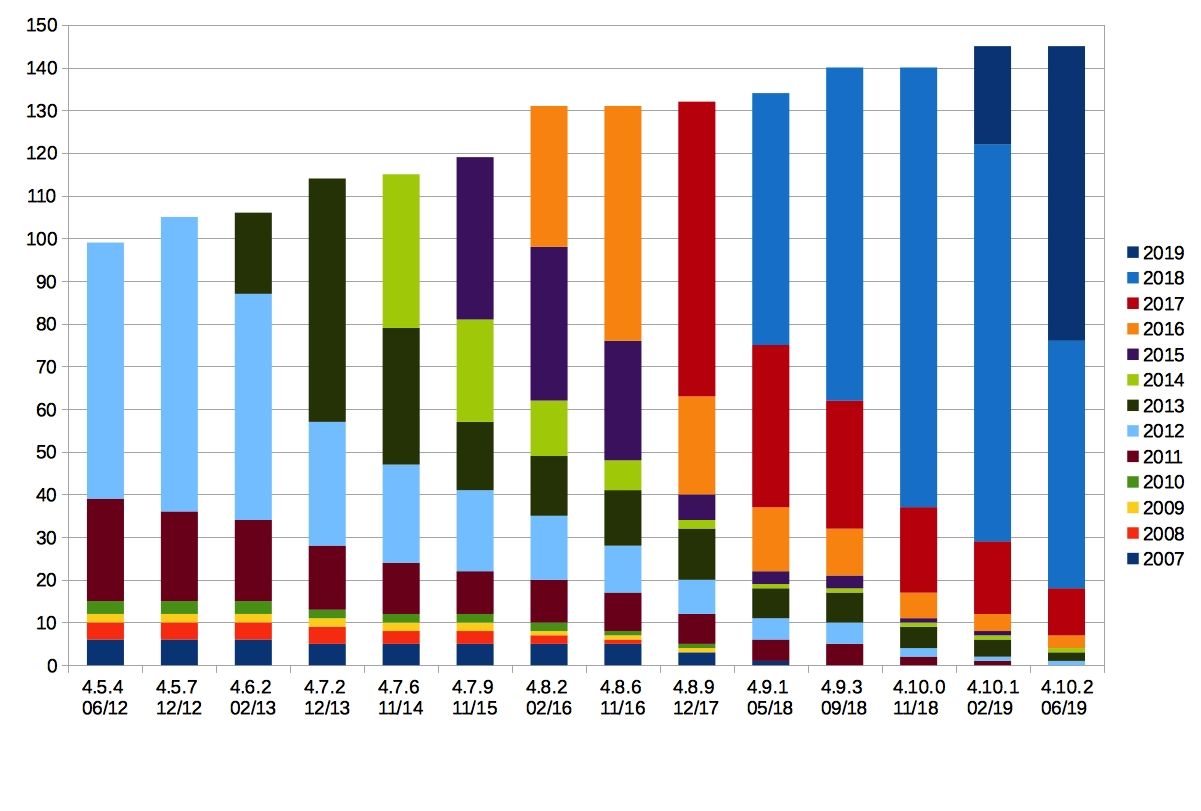
\includegraphics[width=\textwidth]{images/gap-package-releases}
    \caption{Number of GAP packages and their release year}
    \label{fig:gap-package-releases}
\end{figure}

Figure~\ref{fig:gap-package-releases} shows that not only
package releases became more frequent, but also their quality
improved. We are able to tests more packages, and tests pass
for more packages. At the same time, community grows - it
shows the number of package authors.

\begin{figure}[!ht]
    \centering
    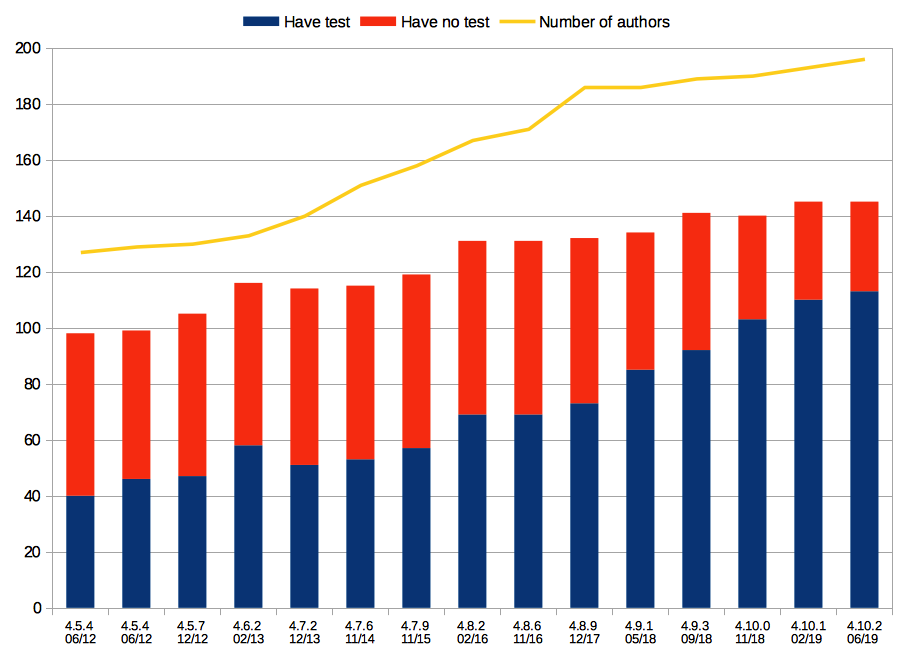
\includegraphics[width=\textwidth]{images/gap-package-tests}
    \caption{Number of GAP packages, their authors, and packages with tests.}
    \label{fig:gap-package-tests}
\end{figure}

\subsection{GAP package manager}\label{pkg-manager}

WHO: Michael

Describe \url{https://gap-packages.github.io/PackageManager/}

\subsection{Packaging GAP distribution}\label{distro}

WHO: Alex

When we decide that there is a time for the next release
(minor or major; update releases were in the past but then abolished).
What are the standards for passing tests. 

How release wrapping is automated.
Which GAP distributions we provide officially.

Figure~\ref{fig:gap-package-releases} shows how package releases became more frequent.

\begin{figure}[!ht]
    \centering
    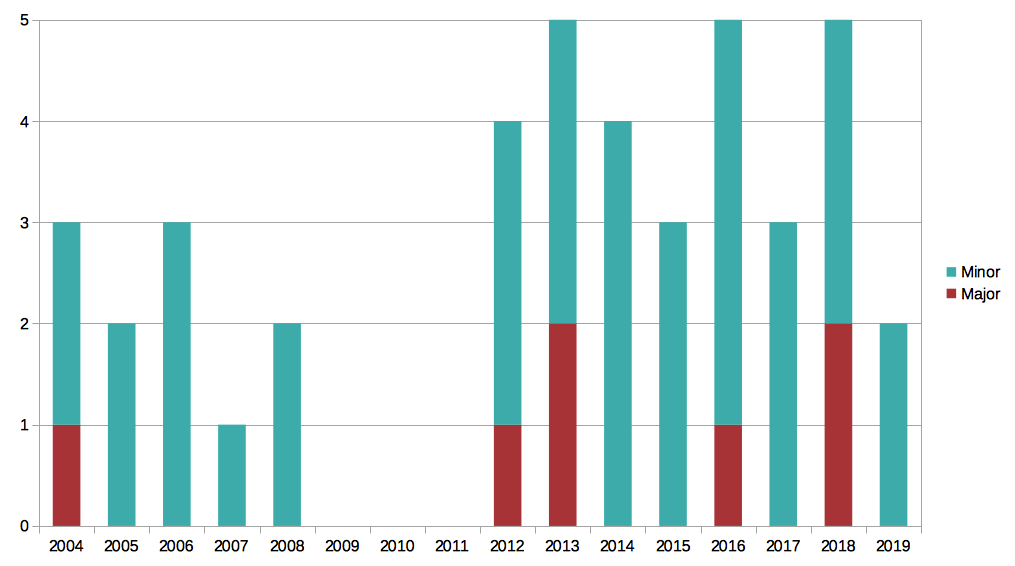
\includegraphics[width=\textwidth]{images/gap-releases}
    \caption{Number of major and minor GAP releases per year since GAP 4.4 release.}
    \label{fig:gap-releases}
\end{figure}

Main distributions
Regression testing
Windows distribution and installer migrated from Windows 7 to Windows 10
Alternative distributions: Docker, Homebrew, 
Opportunity to try GAP online with Jupyter notebook running on Binder.
Improved testing
Code coverage, various sets of automated Travis builds
This is based on Docker containers for various branches.

\section{Jupyter interface to GAP}

WHO: Alex, with help from and Michael

TODO: Refer to previous deliverables and describe how their outputs
evolved and any impacts they achieved

JupyterKernel has been reported in DX.Y. Since that, there were
several more releases of the kernel, associated with new GAP
releases, improving its robustness. 

JupyterKernel lead to several follow-up developments, their
functionality will be described below: Francy, JupyterViz,
other work by Nathan Carter (also mention related work on
GroupExplorer).

Have used in in teaching and in explaining how to share 
reproducible experiments that use GAP. Using Binder
allows to try GAP in Jupyter online. Provide details
and consider including an appendix with an example 
demonstrating the setup.

\section{Community building, Technical support, User Training and Dissemination}\label{gap-support}

WHO: Alex

Describe all training events, Software Carpentry lesson, other workshops

\section{Interfaces, WP6}

WHO: Michael

Fix title of the section.

High-level interoperability

Persistent memoisation

\section{A collection of demonstrators}

For example:

Reproducible experiments with Jupyter

``full-stack semigroups''

persistent memoisation

databases

% TODO: Bibliography. Ensure that we are following software citation recommendations properly!
\end{document}


%%% Local Variables:
%%% mode: latex
%%% TeX-master: t
%%% End:

